%%% The BEGINNING ~~~~~
%%
% ~ Writes Y150239Genomics--SI by George Pacheco.

%% Preamble Settings %%

% Defines document class and paper size ~
\documentclass[twoside, british, a4paper]{article}
\usepackage[paper=portrait, pagesize]{typearea}

\usepackage{amsmath}
\usepackage{amsfonts}
\usepackage{amssymb,upref}
\usepackage{tgheros}
\usepackage{tgtermes}
\usepackage{anyfontsize}
\usepackage{enumitem}
\usepackage{siunitx}
\usepackage{balance}
\usepackage{float}
\usepackage{pdflscape}
\usepackage[nottoc]{tocbibind}
\usepackage{academicons}
\usepackage{array}


\usepackage{subfigure}
\usepackage[subfigure]{tocloft}
\setlength\cftbeforefigskip{20pt}
\cftsetindents{fig}{0pt}{0pt}

% Fixes margins ~
\usepackage{geometry}
\geometry{reset, ignoreall,
  textheight = 253mm,
  textwidth = 175mm,
  bottom = 21mm,
  inner = 17.5mm,
  footskip = 8mm,
  headsep = 5mm,
  headheight = 10pt}
\usepackage[utf8]{inputenc}
\usepackage{fancyhdr}
\renewcommand{\headrule}{}
\renewcommand{\footrule}{}

\setlength{\skip\footins}{1.75pc plus 5pt minus 2pt}
\def\footnoterule{
\kern-3mm \hrule height .5pt \kern -.4pt 
\kern 1mm}

\pagestyle{fancy}
\fancyhead[L]{Y150239 Genomics}
\fancyhead[R]{Pacheco et al. 2024}
\fancypagestyle{firstpage}{%
\fancyhf{}
\lhead{}
\rhead{}}


\fancypagestyle{mylandscape}{
\fancyhf{} %Clears the header/footer
\fancyfoot{% Footer
\makebox[\textwidth][r]{% Right
  \rlap{\hspace{.75cm}% Push out of margin by \footskip
    \smash{% Remove vertical height
      \raisebox{4.87in}{% Raise vertically
        \rotatebox{90}{\thepage}}}}}}% Rotate counter-clockwise
\renewcommand{\headrulewidth}{0pt}% No header rule
\renewcommand{\footrulewidth}{0pt}% No footer rule
}

% Loads packages for images ~
\usepackage{graphicx}
\usepackage{rotating}

% Loads packages for comments ~
\usepackage{verbatim}
\usepackage[hang, flushmargin]{footmisc}

% Loads packages for tables ~
\usepackage{float}
\usepackage{multirow}
\usepackage{charter}
\usepackage{textcomp}
\usepackage[utf8]{inputenc}

% Listing of source code ~
\usepackage{listings}
\usepackage{color}
\definecolor{dkgreen}{rgb}{0,0.6,0}
\definecolor{gray}{rgb}{0.5,0.5,0.5}
\definecolor{mauve}{rgb}{0.58,0,0.82}
\lstset{
  frame = tb,
  language = sh,
  aboveskip = 3mm,
  belowskip = 3mm,
  showstringspaces = false,
  columns = flexible,
  basicstyle = {\small\ttfamily},
  numbers = none,
  numberstyle = \tiny\color{gray},
  keywordstyle = \color{blue},
  commentstyle = \color{dkgreen},
  stringstyle = \color{mauve},
  breaklines = true,
  breakatwhitespace = true,
  tabsize = 3}
  
% Changes caption starting text ~
\renewcommand{\listfigurename}{List of Supplementary Figures}
\renewcommand{\figurename}{}
\renewcommand{\tablename}{}

% Loads packages for typing ~
\usepackage{lettrine}
\pdfmapfile{=montserrat.map} 
\renewcommand{\LettrineFont}{
  \fontfamily{Optima}\fontsize{30}{30}\selectfont
  \color[rgb]{.25, .25, .25}}
\usepackage{marvosym}

\newcommand\myhline{\noindent\rule[.5pt]{\linewidth}{.4pt}\par}

\newcommand{\myheaders}[1] {\noindent{\normalsize{\fontfamily{Optima}\selectfont{\textbf{#1}}}}}
\newcommand{\mysubheaders}[1] {\noindent{\fontfamily{Optima}\selectfont{\textbf{#1}}}}
\newcommand{\mytext}[1] {\noindent{\fontfamily{Optima}\selectfont{#1}}}
\newcommand{\mycaptions}[1] {\noindent{\footnotesize{\fontfamily{Optima}\selectfont{#1}}}}

% Figure captions
\usepackage{caption}
\DeclareCaptionFont{Arial}{\footnotesize{\fontfamily{Arial}\selectfont{#1}}}
\DeclareCaptionLabelSeparator{vline}{\;|\;}
\captionsetup{
 labelsep=vline, 
 font={Arial}, 
 labelfont={Arial},
 belowskip=-12pt}
\newcommand{\figurecaption}[2]{\caption[#1]{\textbf{#1.} #2}}
\usepackage{hyperref}
\usepackage[dvipsnames]{xcolor}
\definecolor{mycolor}{HTML}{F7F8E0}
\definecolor{myorange}{RGB}{245,156,74}
\hypersetup{
  colorlinks = true,
  linkcolor = [RGB]{58, 121, 175},
  urlcolor = -myorange}

\usepackage{fontawesome}

\usepackage[nopar]{lipsum}
\newcommand\blfootnote[1]{%
  \begingroup
  \renewcommand\thefootnote{}\footnote{#1}%
  \addtocounter{footnote}{-1}%
  \endgroup}

% Loads packages for bibliography ~
\usepackage[
backend = biber,
style = nature,
sorting = ynt
]{biblatex}
\addbibresource{FPGP--MainText.bib}

\usepackage{blindtext}
\usepackage{multicol}

%% Starts Document %%

\usepackage{chngcntr}
\counterwithin{figure}{section} 
\AtBeginDocument{\counterwithin{lstlisting}{section}}

% Starts document ~
\begin{document}\thispagestyle{empty}

\hfill\break

% Sets title ~
\Large{\bfseries{\fontfamily{Optima}\color[rgb]{.25,.25,.25}\noindent{SUPPLEMENTARY INFORMATION FOR}}} \\

\hfill
\hfill

% Sets title ~
\LARGE{\bfseries{\fontfamily{Optima}\color[rgb]{0,0,0}\noindent{Genomic Data Unveil Genealogy of a Curious Sparrow}}} \\

% Sets authorship ~
\fontfamily{Optima} \small \noindent 
George Pacheco\,$^{1}$\textsuperscript{\faEnvelopeO},
Ruth Fawthrop\,$^{2}$,
Peter de Vries\,$^{1}$,
Glenn-Peter Sætre\,$^{1}$,
Mark Ravinet\,$^{1}$,
Melissah Rowe\,$^{2}$ \\
\myhline

% Add some vertical space to better center the figure
\vspace{3cm}

\begin{figure}[h!]
\centering
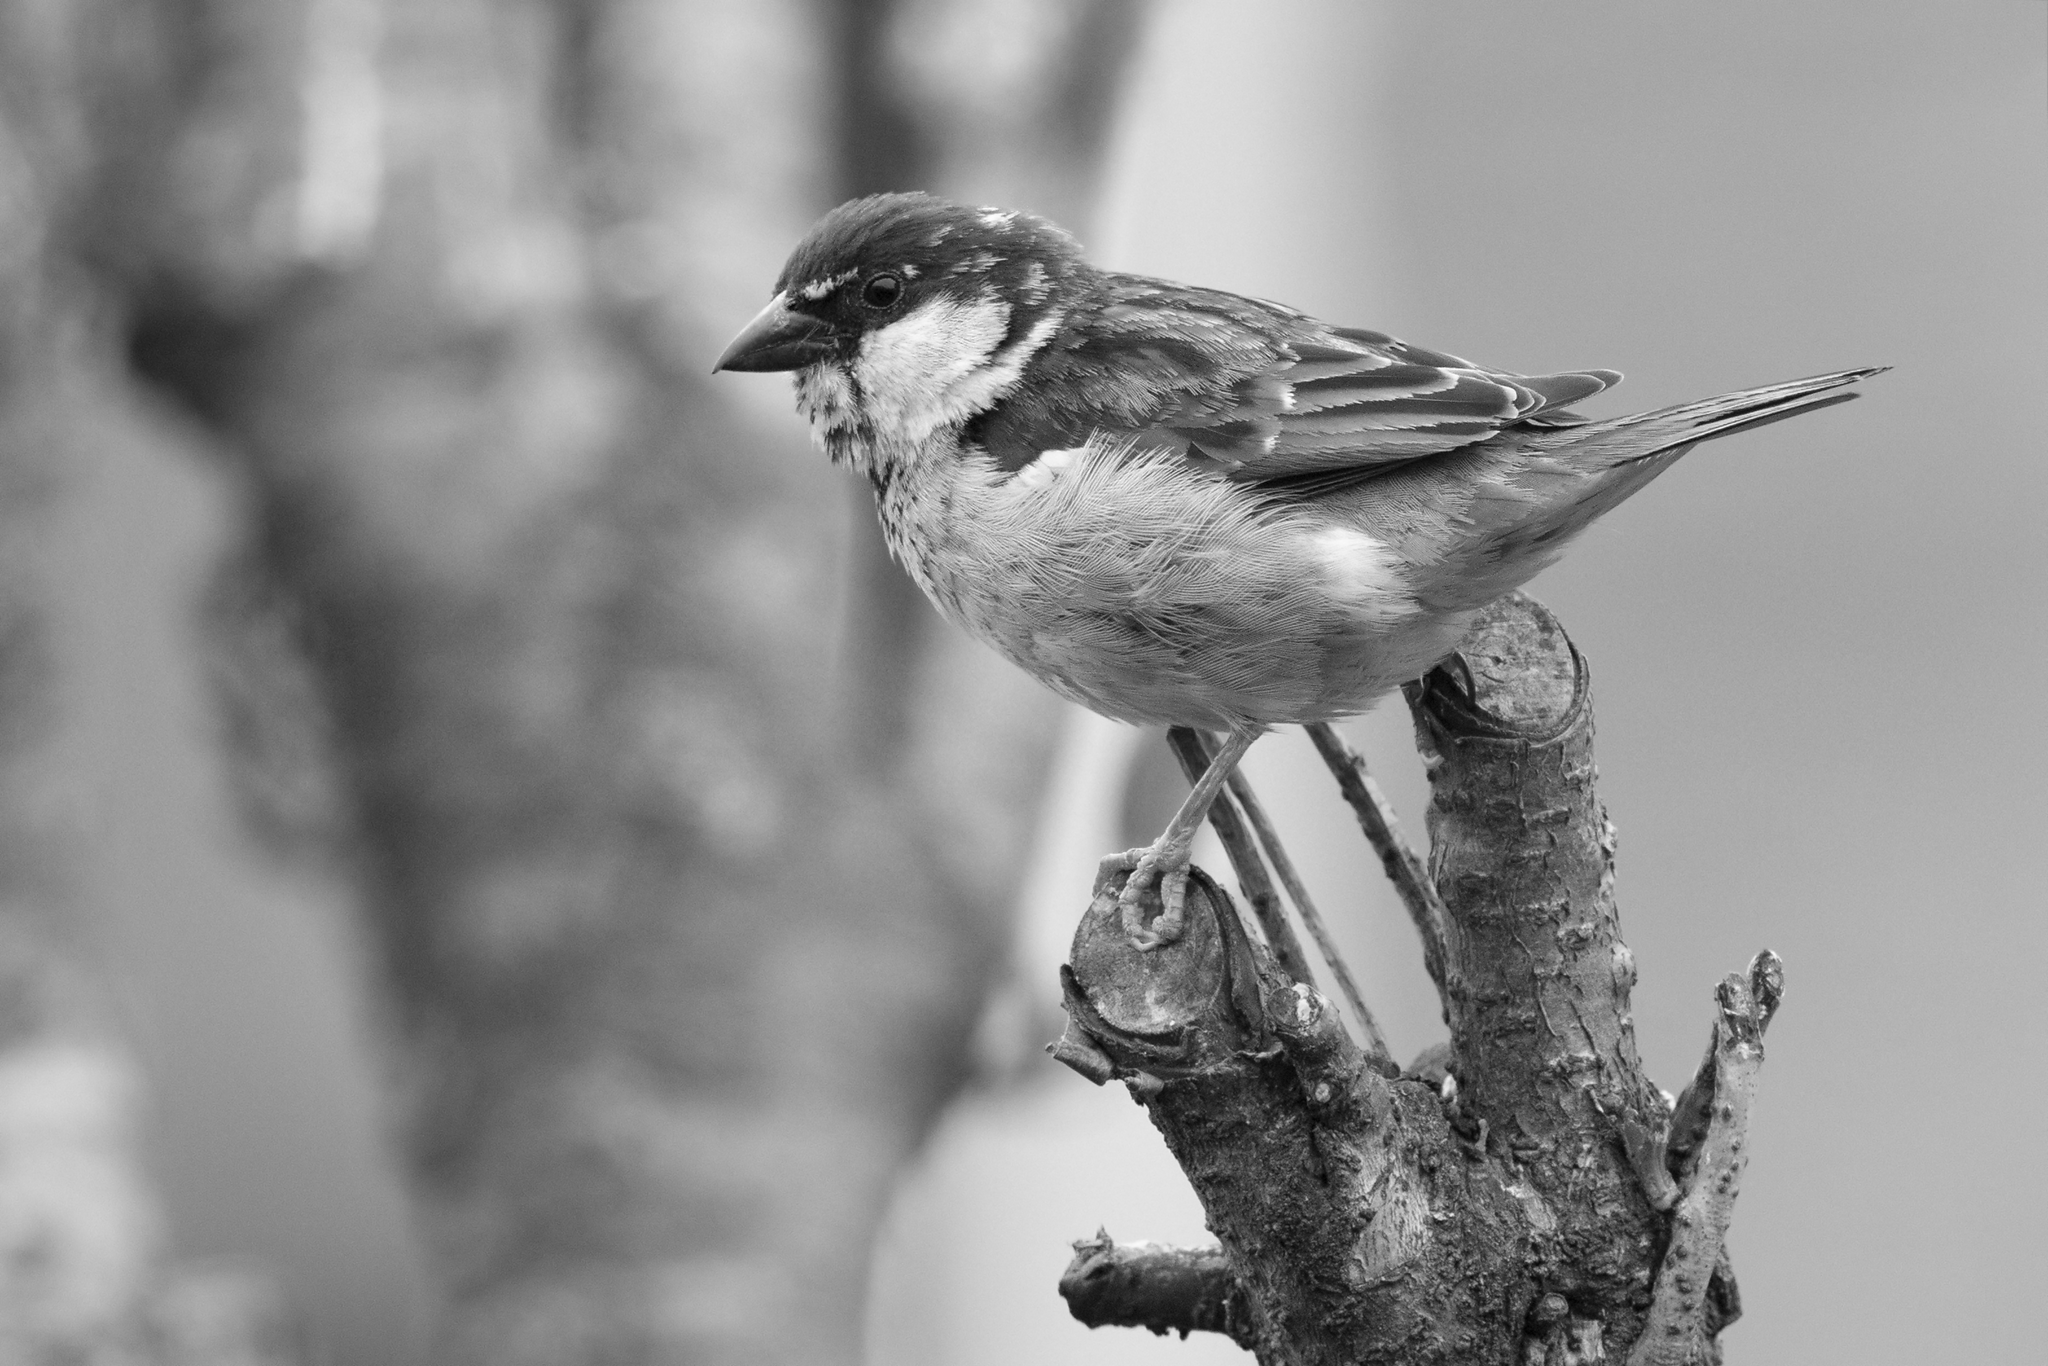
\includegraphics[width=1\textwidth]{./Y150239Genomics_SIPicture.png}
\captionsetup{labelformat=empty}
\label{SI:Y150239Genomics--MeanDepth}
\end{figure}

% Sets affiliations ~
\blfootnote{\scriptsize{\fontfamily{Optima}$^1$Centre for Ecological and Evolutionary Synthesis (CEES), University of Oslo, Oslo, Norway. \\
$^2$Department of Animal Ecology, Netherlands Institute of Ecology (NIOO‐KNAW), Wageningen, The Netherlands. \\
$^3$University of Nottingham, Nottingham, United Kingdom. \\
\textsuperscript{\faEnvelopeO}Correspondence should be addressed to \href{mailto:george.pacheco@ibv.uio.no}{george.pacheco@ibv.uio.no}.}}

\hfill

\newpage
\clearpage

% Table of Contents %

\clearpage
\pagenumbering{roman}
\let\oldnumberline\numberline
\renewcommand{\numberline}[1]{\oldnumberline{}}
\hfill\break
\listoffigures
\let\numberline\oldnumberline
\newpage

\clearpage
\pagenumbering{arabic}

% Example of a table
\begin{table}[h!]
  \centering
  \caption{Sample Table with Borders}
  \begin{tabular}{|p{3cm}|p{3cm}|}
      \hline
      \textbf{Data Set} & \textbf{Description} & \textbf{\# of samples} & \textbf{\# of SNPs} \\
      \hline
      Autosomes I & Autosomic SNP panel not including the out-group (Tree Sparrow). & 69 & 521,612 \\
      \hline
      ChromosomeZ I & Z chromosome SNP panel not including the out-group (Tree Sparrow). & 79 & 2,796 \\
      \hline
      Autosomes II & Autosomic SNP panel not including the out-group (Tree Sparrow). & 79 & 0 \\
      \hline
      ChromosomeZ II & Z chromosome SNP panel not including the out-group (Tree Sparrow). & 79 & 0 \\
      \hline
  \end{tabular}
  \end{table}

\begin{figure}
\centering
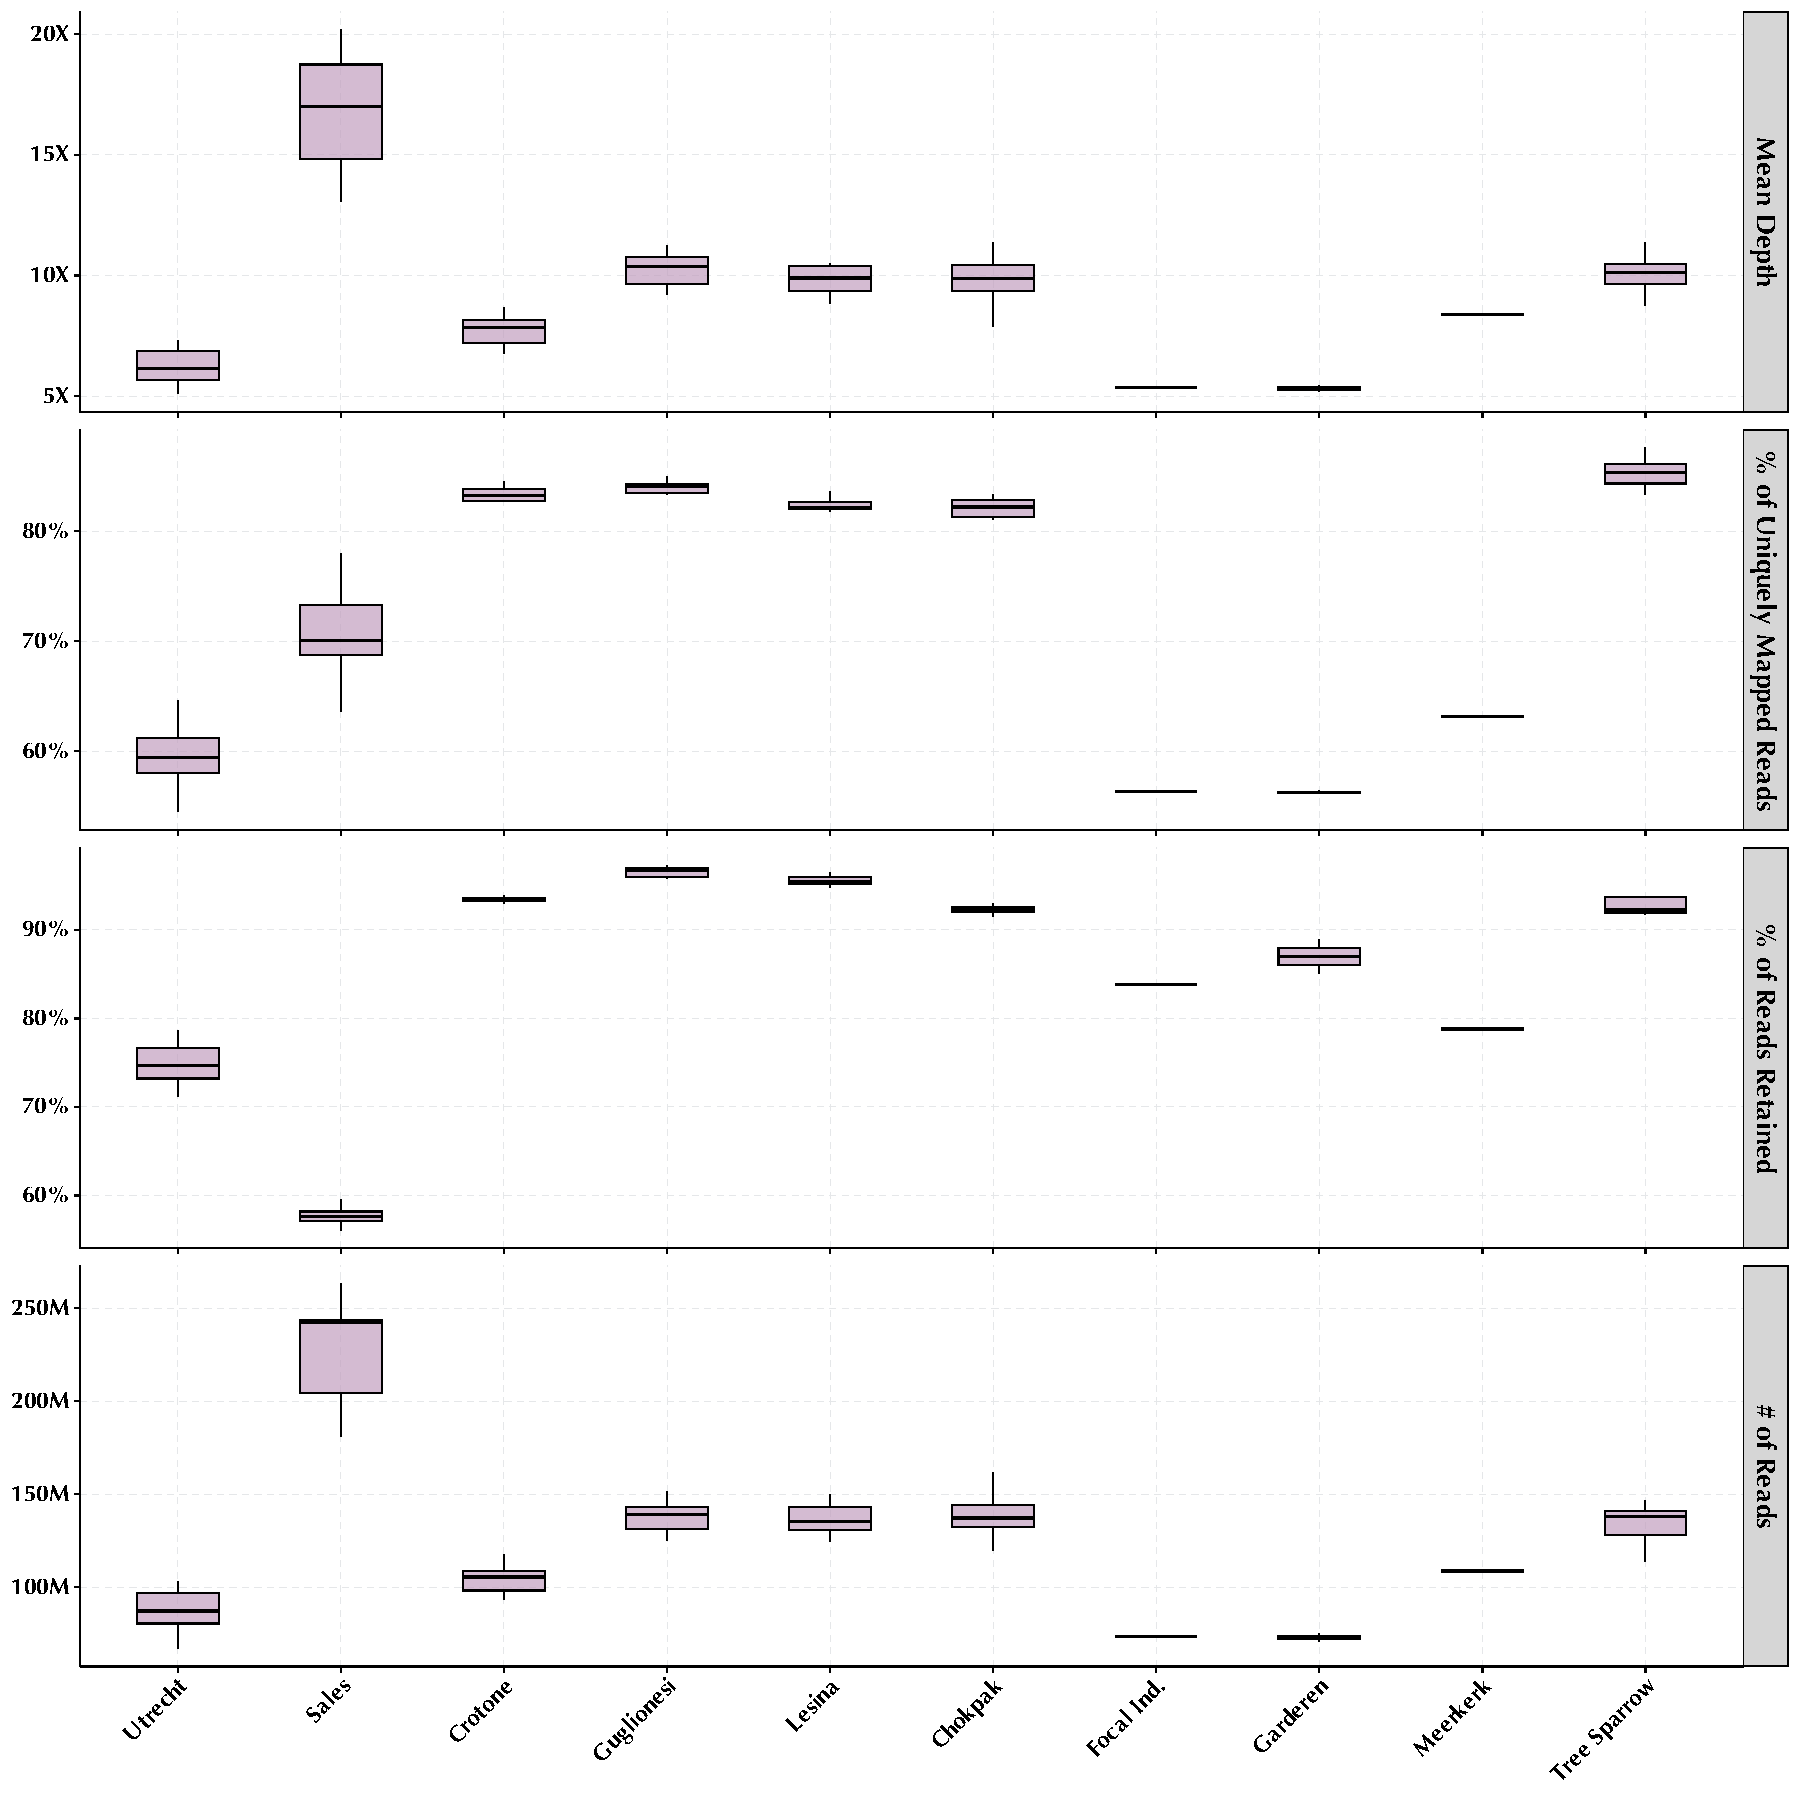
\includegraphics[width=1\textwidth]{../Y150239Genomics--Pipeline/Y150239Genomics--Plots/Y150239Genomics--Stats/Y150239Genomics--Stats.pdf}
\captionsetup{labelformat=empty}
\caption[\textbf{Supplementary Figure 1.}]{\textbf{Supplementary Figure 1.} Boxplots summarising the processing and mapping statistics of the sequencing data analysed grouped by population.}
\label{SI:Y150239Genomics--Stats}
\end{figure}

\begin{figure}
\centering
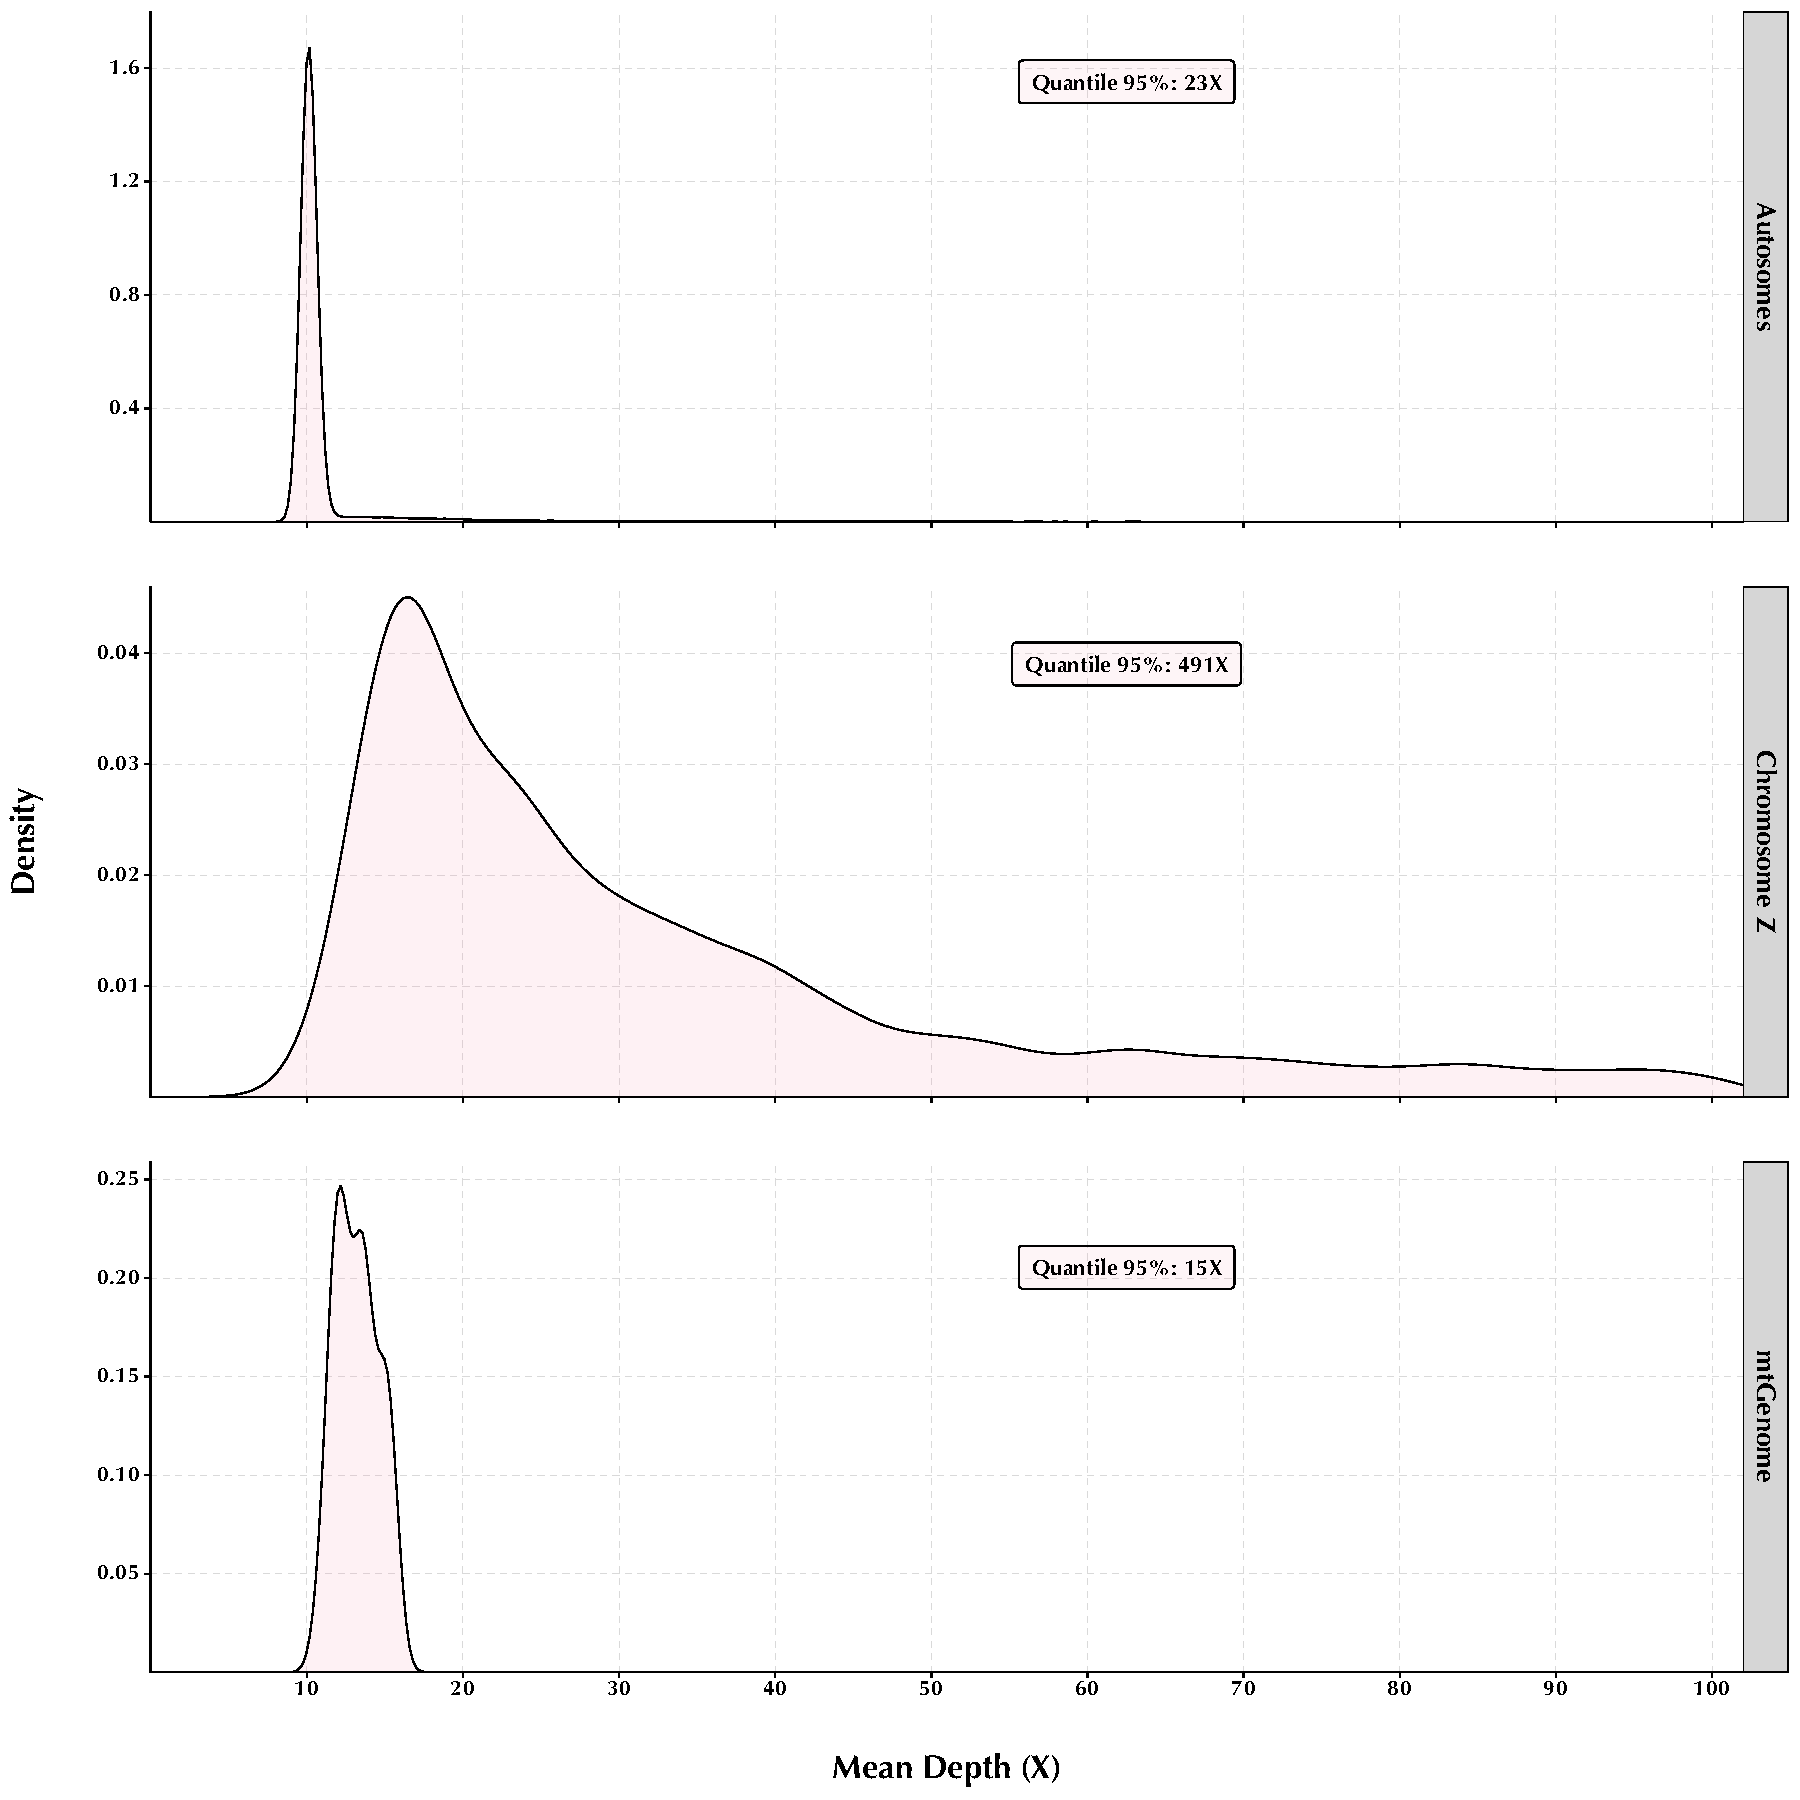
\includegraphics[width=1\textwidth]{../Y150239Genomics--Pipeline/Y150239Genomics--Plots/Y150239Genomics--Stats/Y150239Genomics--MeanDepth.pdf}
\captionsetup{labelformat=empty}
\caption[\textbf{Supplementary Figure 2.}]{\textbf{Supplementary Figure 2.} Density plots summarising the per SNP mean depth across all samples categorised by chromosome type.}
\label{SI:Y150239Genomics--MeanDepth}
\end{figure}

\begin{figure}
\centering
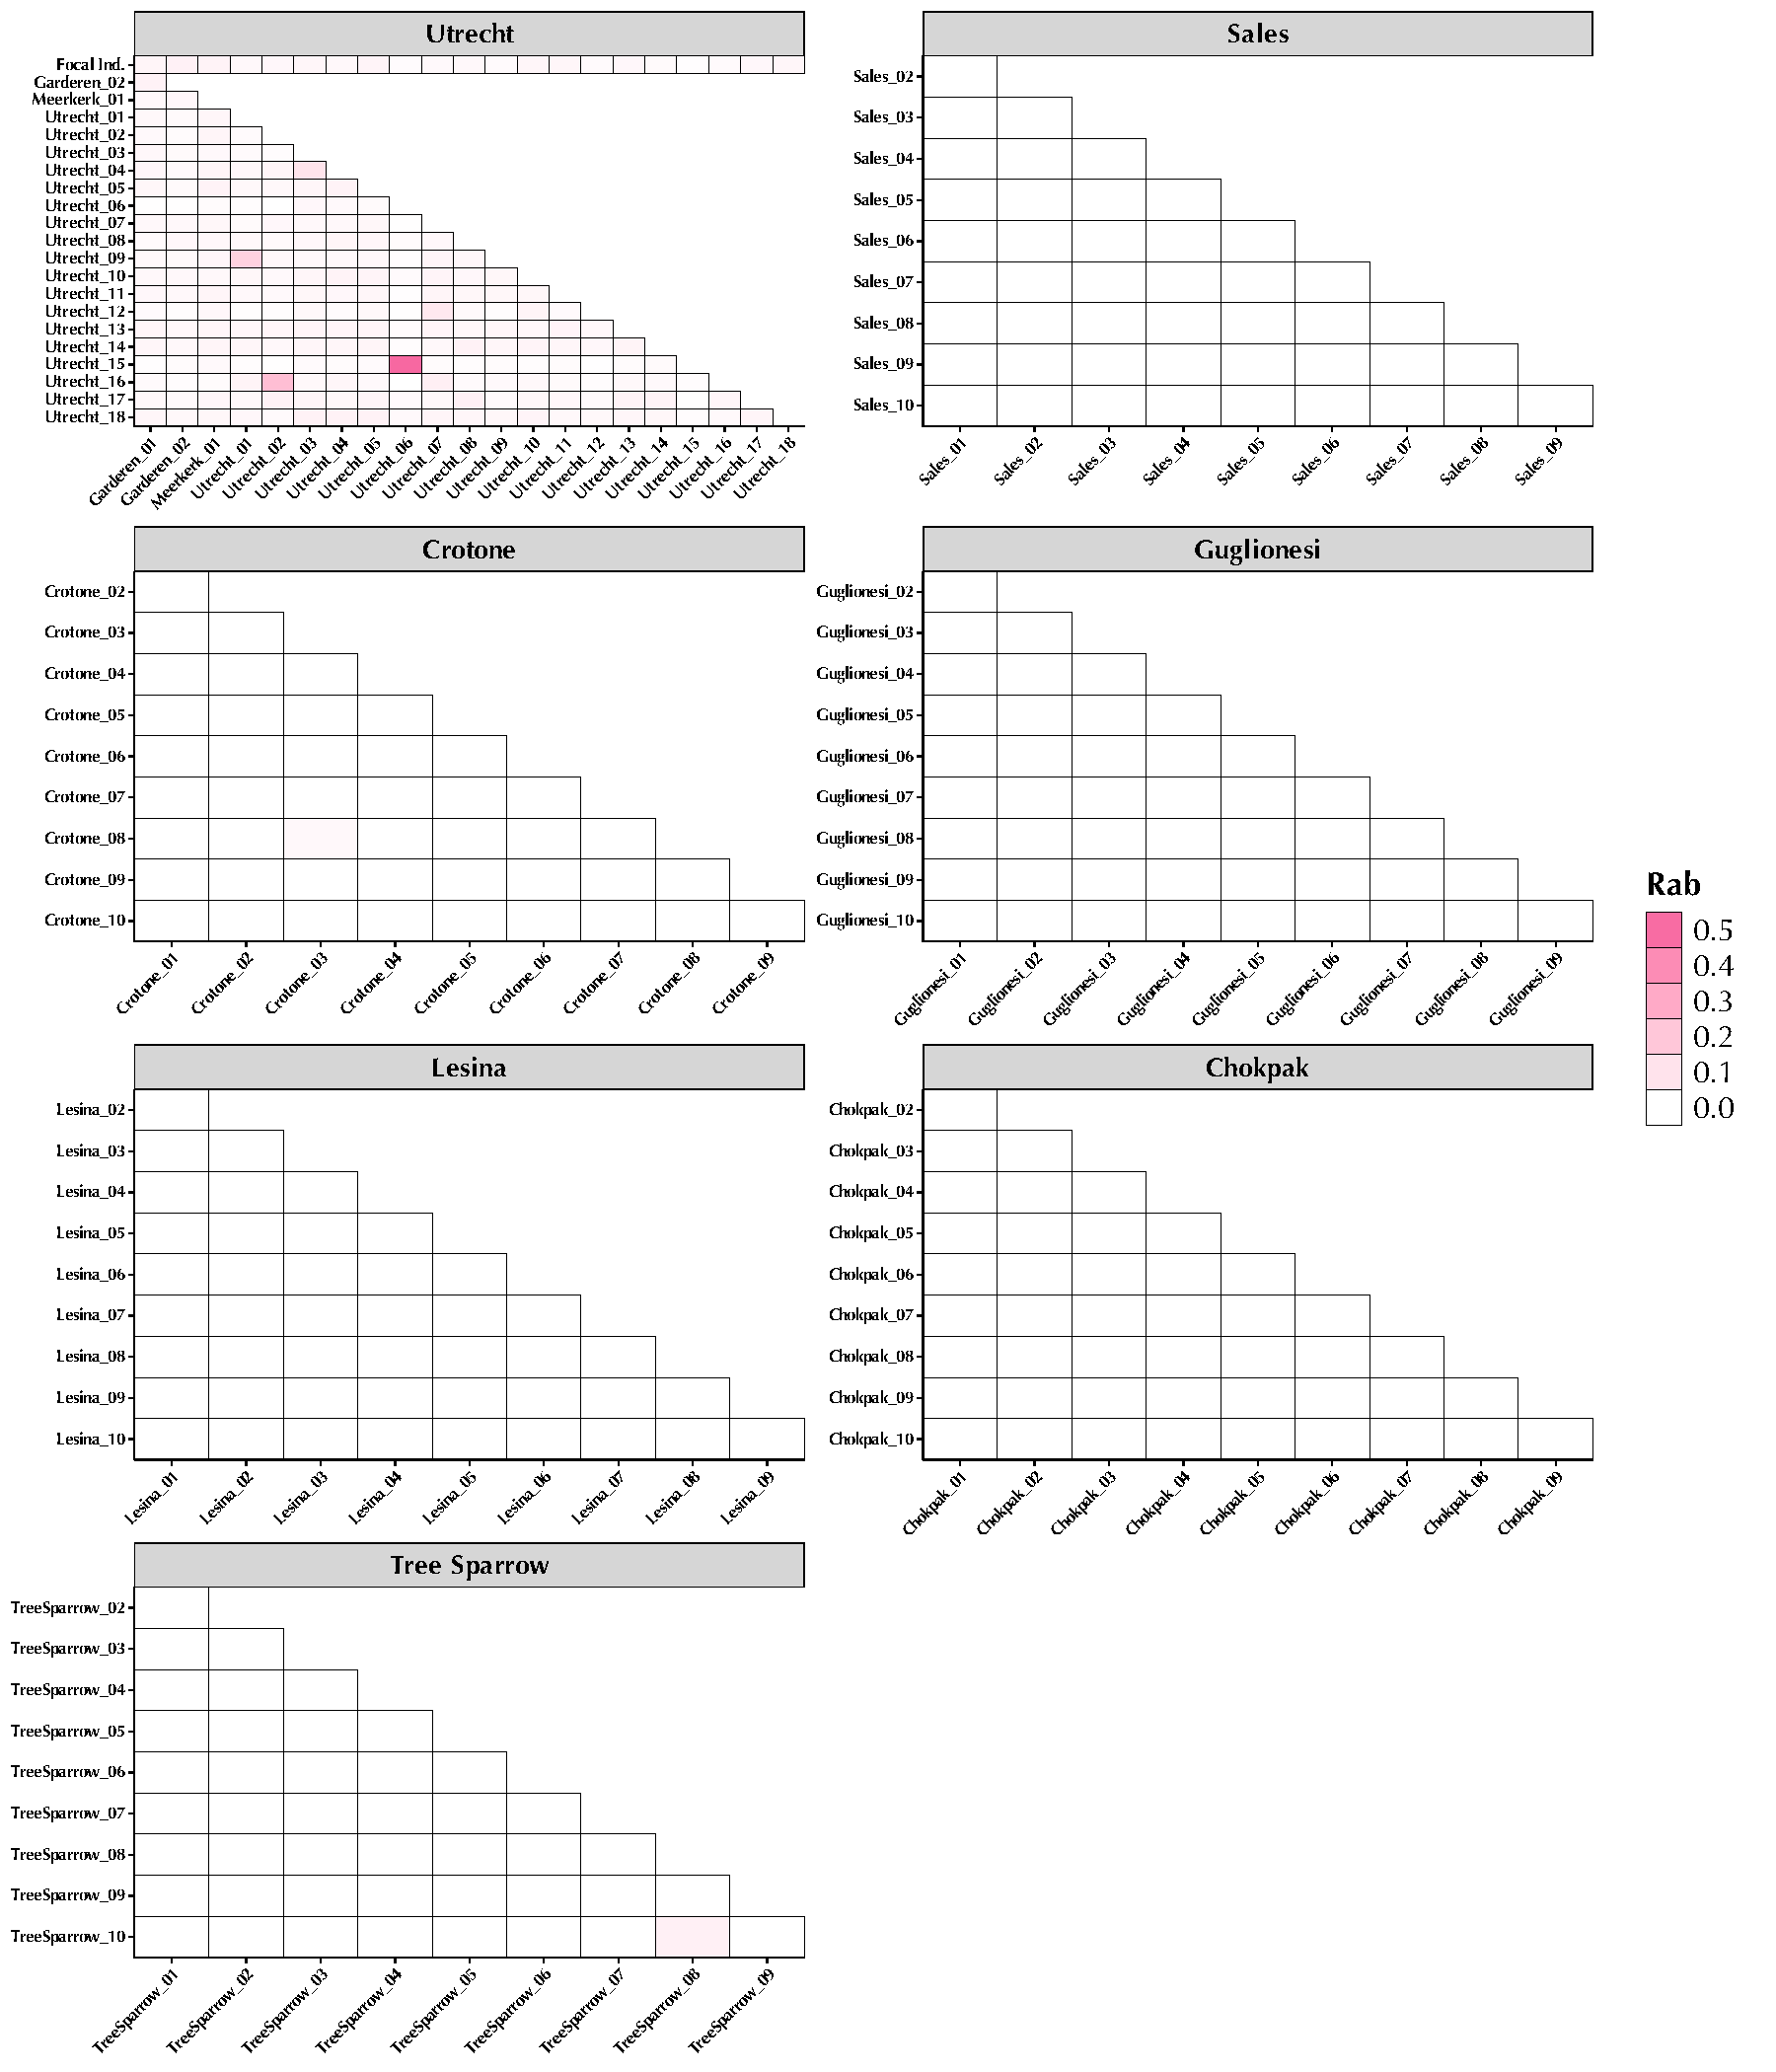
\includegraphics[width=1\textwidth]{../Y150239Genomics--Pipeline/Y150239Genomics--Plots/Y150239Genomics--Kinship/Y150239Genomics--Kinship.pdf}
\captionsetup{labelformat=empty}
\caption[\textbf{Supplementary Figure 3.}]{\textbf{Supplementary Figure 3.} Heat maps of the RAB statistics based on the autosome genomic data grouped by population.}
\label{SI:Y150239Genomics--Kinship}
\end{figure}

\begin{figure}
\centering
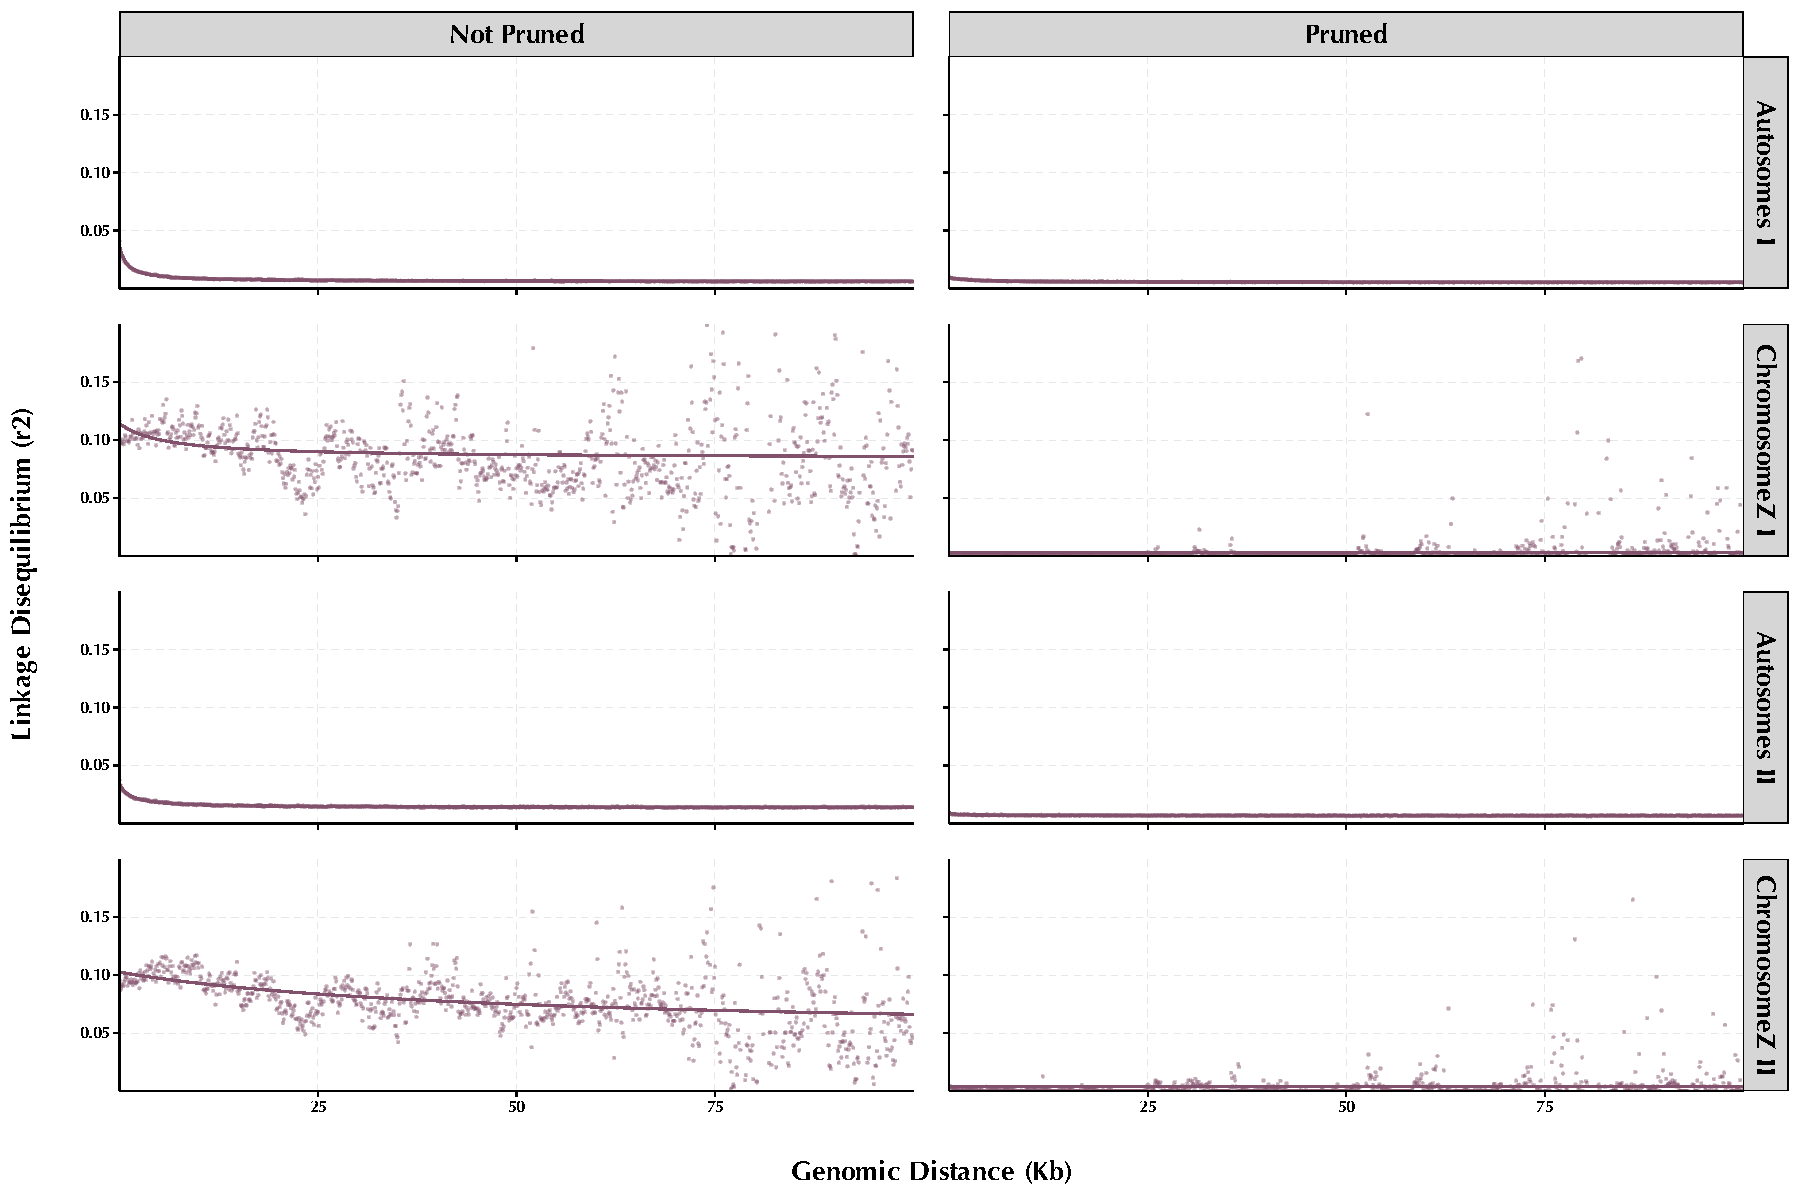
\includegraphics[width=1\textwidth]{../Y150239Genomics--Pipeline/Y150239Genomics--Plots/Y150239Genomics--LD/Y150239Genomics--LD.pdf}
\captionsetup{labelformat=empty}
\caption[\textbf{Supplementary Figure 4.}]{\textbf{Supplementary Figure 4.} Linkage disequilibrium decays calculated individually based on chromosomal classification before and after linkage disequilibrium pruning.}
\label{SI:Y150239Genomics--LD}
\end{figure}

\begin{figure}
\centering
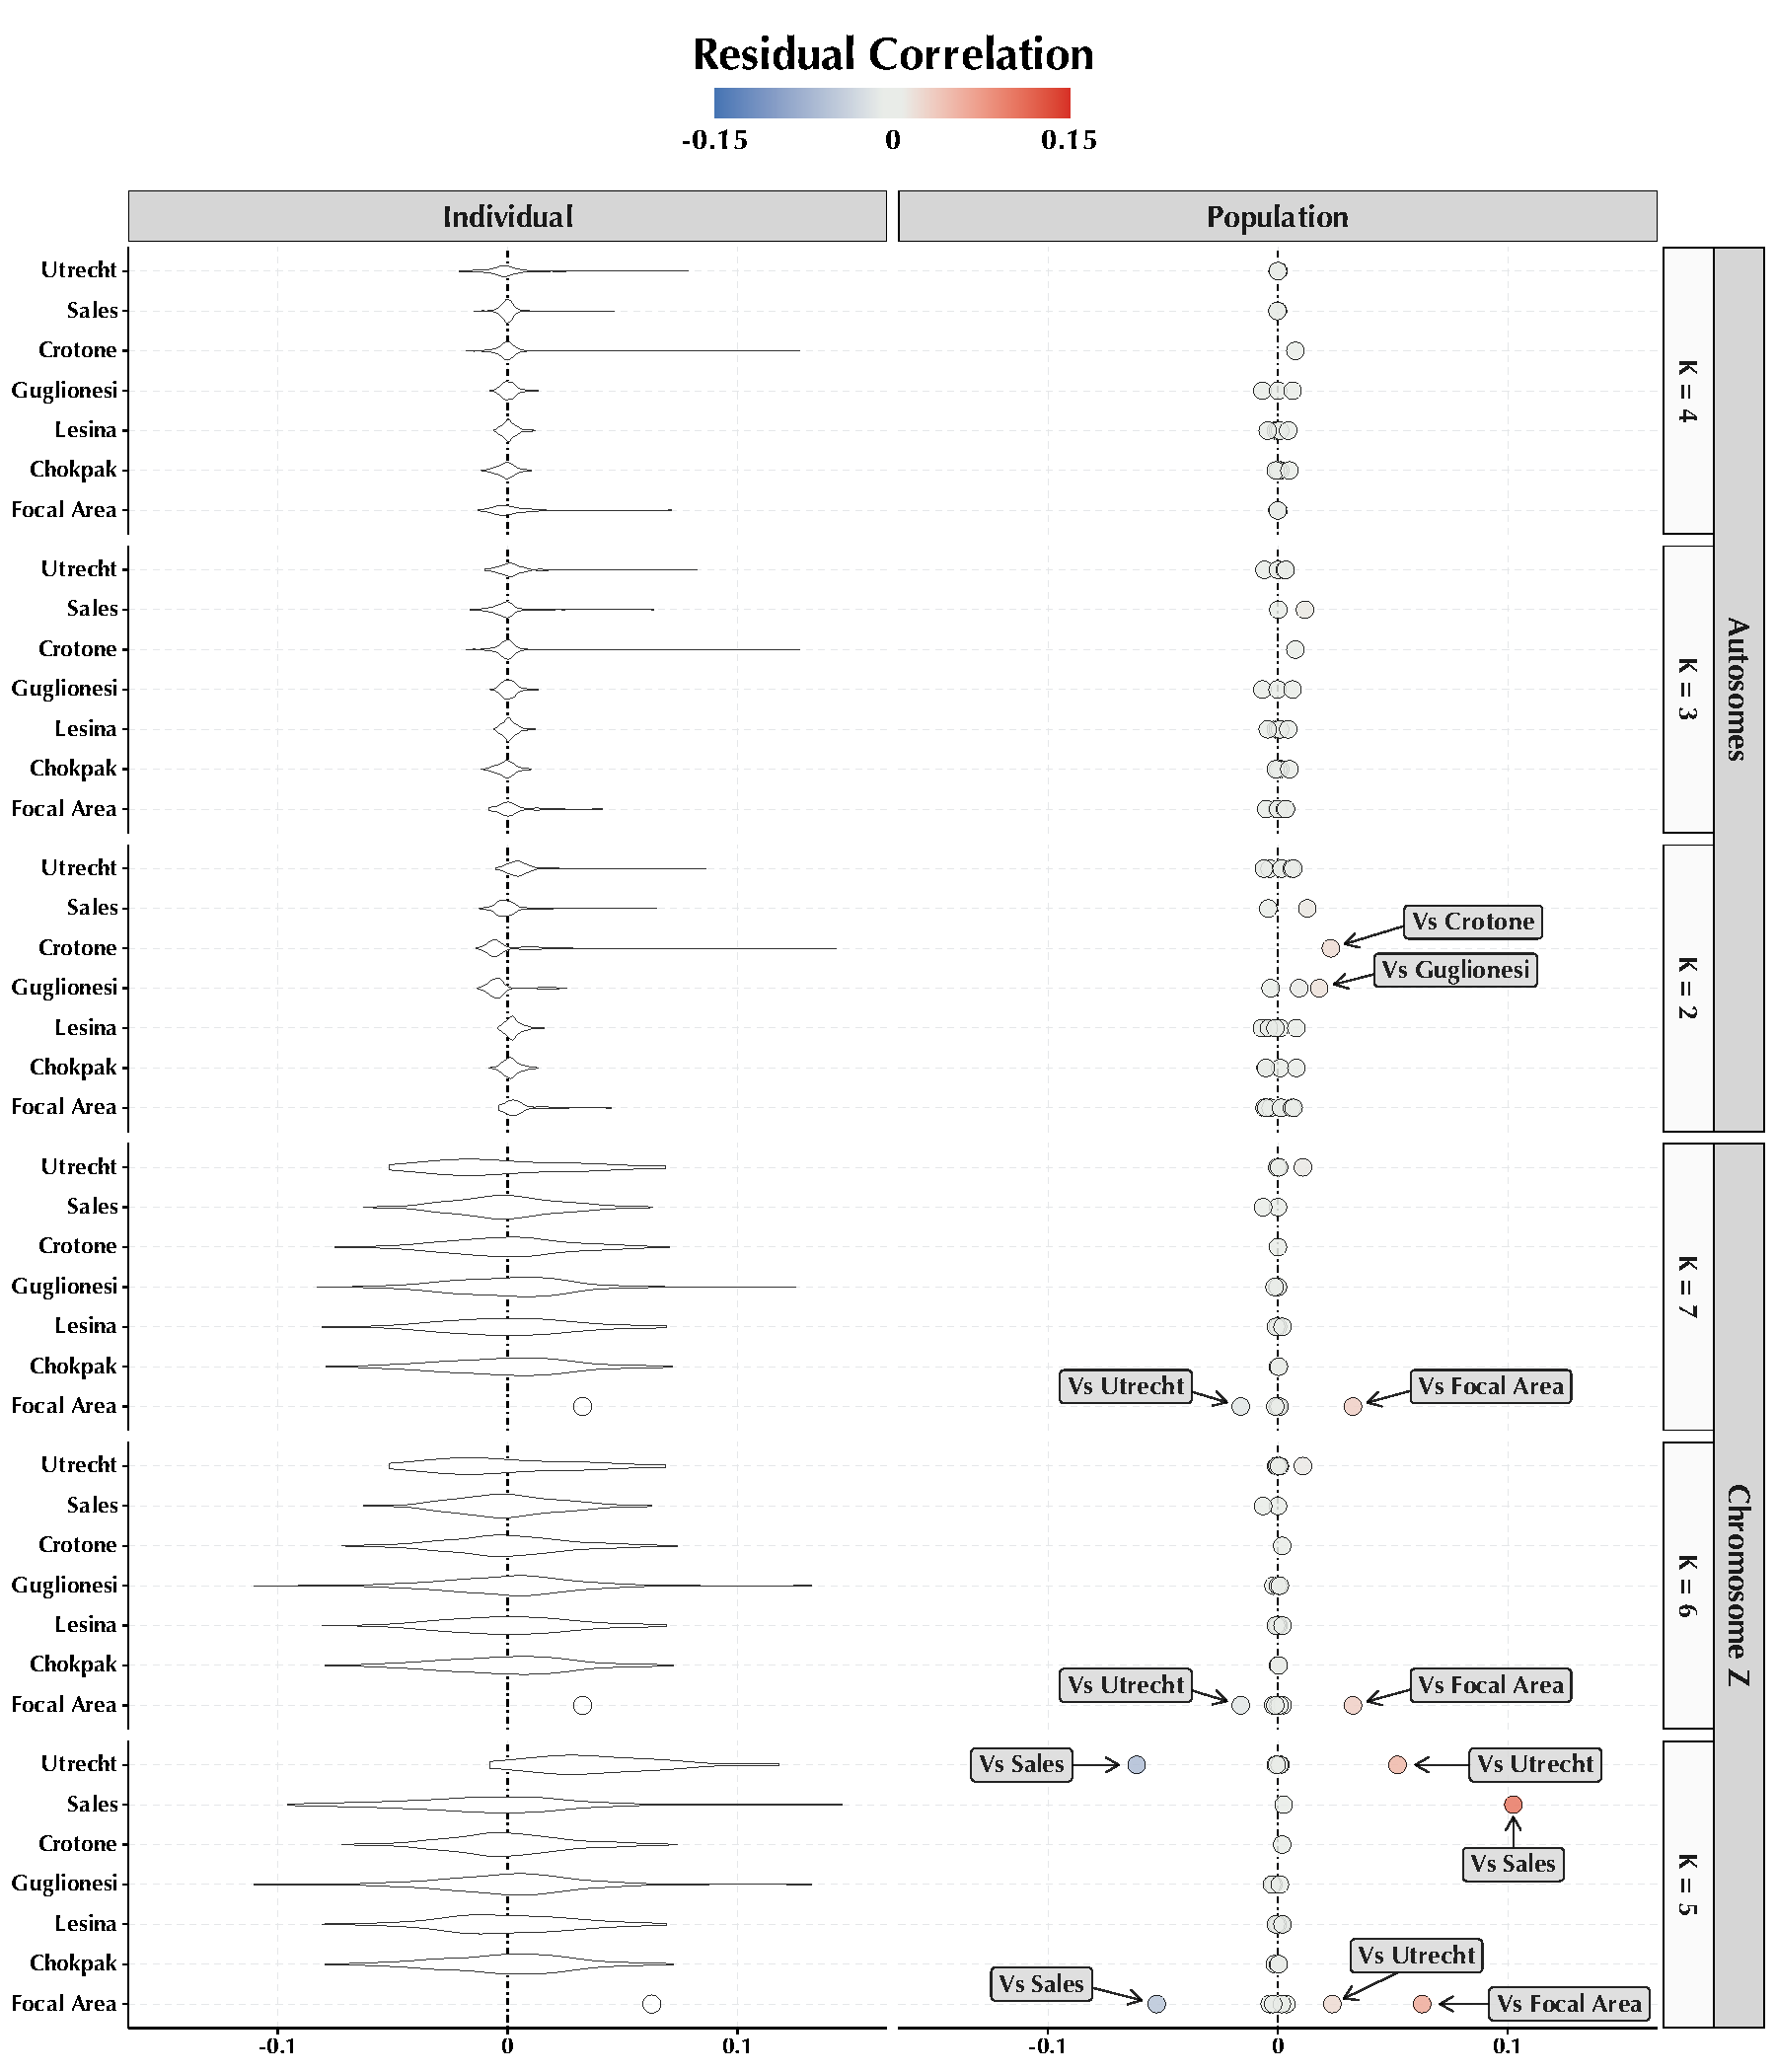
\includegraphics[width=.85\textwidth]{../Y150239Genomics--Pipeline/Y150239Genomics--Plots/Y150239Genomics--ngsAdmix/Y150239Genomics--evalAdmix.pdf}
\captionsetup{labelformat=empty}
\caption[\textbf{Supplementary Figure 5.}]{\textbf{Supplementary Figure 5.} }
\label{SI:Y150239Genomics--evalAdmix}
\end{figure}

\end{document}

% 
%%
%%% The END ~~~~~